% ======================================================================
% 2. BACKGROUND
% Job: the minimum systems theory a pentester needs to reason about the
% attack and to defend every claim in it. Order matters:
% orientation -> identity -> secret -> derivation -> protocol -> carrier
% -> what is left behind.
% ======================================================================
\section{Background: How Windows Authenticates}
\label{sec:background}

Three things have to line up before any of this makes sense: a secret, a protocol that accepts it,
and a service that will take the protocol's word for it.

Two values sit in an account record and they are not interchangeable. The \textbf{NT hash} is MD4
over the UTF-16LE password: sixteen bytes, no salt, no iteration count, and identical on every
machine for the same password. The \textbf{LM hash} is the older construction, the password
uppercased, cut to fourteen characters, split into two seven-byte halves and used as DES keys. It
is absent by default on current systems and gives you nothing the NT hash does not. When this
article says ``the hash'', it means the NT hash.

Two protocols consume it. \textbf{NTLM} is challenge-response: the server sends a challenge, the
client computes a response from the hash, the server checks that response against its own copy.
\textbf{Kerberos} is ticket-based: the client asks a KDC, which on a domain is a domain
controller, for a ticket, and under RC4-HMAC the key it proves possession with is the NT hash
itself. Neither puts the hash on the wire. A captured exchange is something to crack offline, not
something to log in with.

A hash or a ticket is worth only what accepts it, and Windows spreads that acceptance over a set of
services rather than one remote-access protocol. Table~\ref{tab:services} lists the ones an
engagement meets, what each is for, and what a valid logon buys there.

Each of these borrows the same authentication layer, which is why one hash reaches all of them and
why blocking a port moves the path rather than closing it.

\begin{table}[htbp]
\centering
\small
\renewcommand{\arraystretch}{1.25}
\caption{Services, and what a valid logon buys on each.}
\label{tab:services}
\begin{tabularx}{\textwidth}{@{}>{\raggedright\arraybackslash}m{2.2cm}>{\raggedright\arraybackslash}m{2.6cm}>{\raggedright\arraybackslash}m{4.2cm}Y@{}}
\toprule
Service & Port & What it is for & A valid logon buys \\
\midrule
\rowcolor{gray!7} SMB & 445 & files and printers & share access, and execution via the service control manager \\
\addlinespace[3pt]
\rowcolor{white} MSRPC & 135 + dynamic & remote procedure calls & service creation, scheduled tasks, DCOM \\
\addlinespace[3pt]
\rowcolor{gray!7} WMI & over MSRPC & system management & process creation, queries \\
\addlinespace[3pt]
\rowcolor{white} WinRM & 5985, 5986 & management over HTTP & command execution without a share \\
\addlinespace[3pt]
\rowcolor{gray!7} RDP & 3389 & an interactive desktop & a desktop session \\
\addlinespace[3pt]
\rowcolor{white} LDAP & 389, 636 & directory queries & reads, and the writes its ACL allows \\
\addlinespace[3pt]
\rowcolor{gray!7} MSSQL & 1433 & a database & queries; \texttt{xp\_cmdshell} with sysadmin \\
\bottomrule
\end{tabularx}
\end{table}

NetBIOS is the layer people misplace. It is a session and naming interface from the LAN Manager
era, not an authentication protocol: SMB once rode on it over TCP 139, and modern SMB runs
directly on 445. What survives is the name service, which is why NBT-NS spoofing still works on
networks that have moved on everywhere else, and why LLMNR, the protocol that took the same job
over, deserves the same treatment.

\subsection{Accounts, SIDs, and the access token}
\label{sec:accounts}

Windows keeps two account databases, and they store the same kind of record. The SAM hive on every
workstation and member server holds the local accounts; \texttt{NTDS.dit} on a domain controller
holds the domain's. Both key an account by a security identifier, a domain or machine SID followed
by a relative identifier, and both keep the account's NT hash beside it
(Figure~\ref{fig:two-stores}). The name is only how people refer to the account. The SID is what
every access check, ACL entry and log line uses, which is why renaming an account changes nothing
and recreating one produces a different identity.

% Figure: one account record, held in the SAM hive or in NTDS.dit.
% Used in section 2.1. Values are illustrative, not taken from a real host.
% Two complete cards, not two columns of one table: each store shows only the
% fields it keeps. The grey band crosses both cards and the gap because the
% rows it covers are the fields both stores hold, at the same height.
\begin{figure}[H]
\centering
\footnotesize
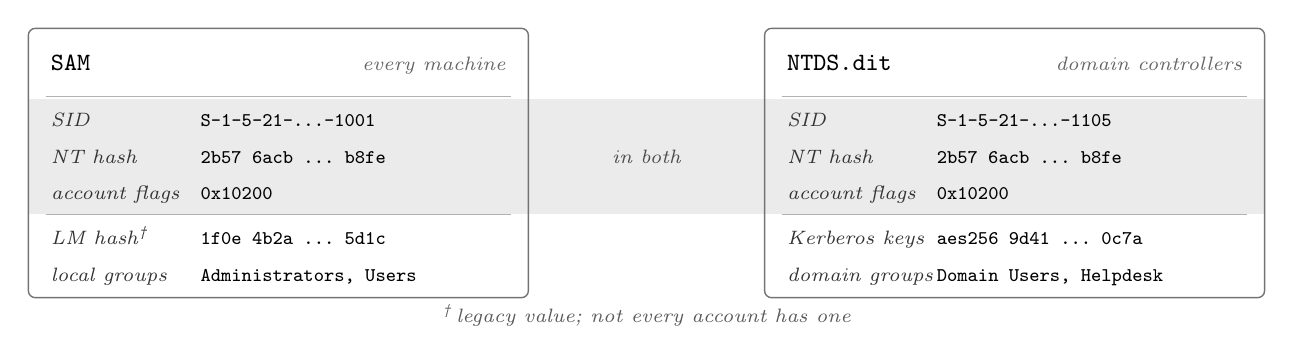
\begin{tikzpicture}[x=1cm,y=1cm,
  card/.style={draw=black!55, line width=0.5pt, rounded corners=2.5pt},
  head/.style={font=\small\ttfamily\bfseries, anchor=base west, inner sep=0pt},
  scope/.style={font=\scriptsize\itshape, text=black!60, anchor=base east,
                inner sep=0pt},
  field/.style={font=\scriptsize\itshape, text=black!80, anchor=base west,
                inner sep=0pt},
  val/.style={font=\scriptsize\ttfamily, anchor=base west, inner sep=0pt}
]

% the shared fields: one band, drawn first so it runs behind both cards
\fill[black!8] (0,-0.90) rectangle (15.7,-2.36);

% the two cards
\draw[card] (0,0) rectangle (6.35,-3.42);
\draw[card] (9.35,0) rectangle (15.7,-3.42);

% header rules and the rule that closes the shared block
\draw[black!30, line width=0.4pt] (0.22,-0.86) -- (6.13,-0.86);
\draw[black!30, line width=0.4pt] (9.57,-0.86) -- (15.48,-0.86);
\draw[black!30, line width=0.4pt] (0.22,-2.36) -- (6.13,-2.36);
\draw[black!30, line width=0.4pt] (9.57,-2.36) -- (15.48,-2.36);

% card headings: store, and the scope it covers
\node[head]  at (0.28,-0.53) {SAM};
\node[scope] at (6.07,-0.53) {every machine};
\node[head]  at (9.63,-0.53) {NTDS.dit};
\node[scope] at (15.42,-0.53) {domain controllers};

% the band's label sits in the gap, on the band itself
\node[font=\scriptsize\itshape, text=black!70, anchor=base]
  at (7.85,-1.71) {in both};

% ---- left card: local account, SAM hive ------------------------------
\node[field] at (0.28,-1.25) {SID};
\node[val]   at (2.18,-1.25) {S-1-5-21-\dots-1001};
\node[field] at (0.28,-1.71) {NT hash};
\node[val]   at (2.18,-1.71) {2b57 6acb \dots\ b8fe};
\node[field] at (0.28,-2.17) {account flags};
\node[val]   at (2.18,-2.17) {0x10200};

\node[field] at (0.28,-2.75) {LM hash\smash{\textsuperscript{\dag}}};
\node[val]   at (2.18,-2.75) {1f0e 4b2a \dots\ 5d1c};
\node[field] at (0.28,-3.21) {local groups};
\node[val]   at (2.18,-3.21) {Administrators, Users};

% ---- right card: domain account, NTDS.dit ----------------------------
\node[field] at (9.63,-1.25) {SID};
\node[val]   at (11.53,-1.25) {S-1-5-21-\dots-1105};
\node[field] at (9.63,-1.71) {NT hash};
\node[val]   at (11.53,-1.71) {2b57 6acb \dots\ b8fe};
\node[field] at (9.63,-2.17) {account flags};
\node[val]   at (11.53,-2.17) {0x10200};

\node[field] at (9.63,-2.75) {Kerberos keys};
\node[val]   at (11.53,-2.75) {aes256 9d41 \dots\ 0c7a};
\node[field] at (9.63,-3.21) {domain groups};
\node[val]   at (11.53,-3.21) {Domain Users, Helpdesk};

% honesty about the legacy value, without cluttering either card
\node[font=\scriptsize\itshape, text=black!65, anchor=base]
  at (7.85,-3.74)
  {\textsuperscript{\dag}\,legacy value; not every account has one};

\end{tikzpicture}
\caption{One account record, two homes.}
\label{fig:two-stores}
\end{figure}


A handful of relative identifiers are fixed, and worth recognising on sight:

\begin{itemize}[leftmargin=1.6em]
  \item \textbf{500} --- the built-in Administrator, on a workstation and on a domain alike.
  \item \textbf{501} --- Guest.
  \item \textbf{502} --- krbtgt, the account whose key encrypts every ticket-granting ticket.
  \item \textbf{512} --- Domain Admins.
  \item \textbf{513} --- Domain Users.
  \item \textbf{515} --- Domain Computers.
\end{itemize}

Everything else starts at 1000 and is issued in order, so the RID of a service account tells you
roughly when it was created.

The logon itself is run by LSASS. \texttt{lsass.exe} is a user-mode process, and the LSA is the
subsystem inside it rather than a second process. The subsystem holds the policy engine, the audit
trail and the table of logon sessions, and builds a token when authentication succeeds. It also
loads the LSA-side instance of each authentication package as a DLL, \texttt{msv1\_0} for NTLM and
the Kerberos package among them, together with the code that reads SAM and the SECURITY hive
(Figure~\ref{fig:lsa-stack}). Callers reach those packages through SSPI, which presents the same
interface to \texttt{winlogon.exe}, to a service, and to your shell.

% Figure: who authenticates, and who authorises. Used in section 2.1.
% Colour carries meaning: blue = process, teal = LSA subsystem, orange =
% authentication package, grey = kernel component. Keep it that way.
\begin{figure}[htbp]
\centering
\small
\begin{tikzpicture}[
  proc/.style={draw=black!45, fill=blue!8, rounded corners=2pt, align=center,
               font=\scriptsize, minimum height=0.72cm},
  api/.style={draw=black!45, fill=white, dashed, align=center, font=\scriptsize,
              minimum height=0.6cm},
  sub/.style={draw=black!45, fill=teal!10, align=center, font=\scriptsize,
              minimum height=0.62cm},
  pkg/.style={draw=black!60, fill=orange!22, align=center, font=\scriptsize,
              minimum height=0.62cm},
  kern/.style={draw=black!45, fill=black!12, align=center, font=\scriptsize,
               minimum height=0.8cm},
  arr/.style={-{Stealth[length=1.8mm]}, draw=black!55, thick}
]

% callers -----------------------------------------------------------
\node[proc, text width=2.6cm] (w) at (1.5,0) {\texttt{winlogon.exe}};
\node[proc, text width=2.2cm] (s) at (4.2,0) {\texttt{services.exe}};
\node[proc, text width=2.4cm] (a) at (6.9,0) {applications};

% the interface every caller uses -----------------------------------
\node[api, text width=6.6cm] (sspi) at (4.2,-1.15) {SSPI \textperiodcentered{} Negotiate};

\draw[arr] (1.5,-0.4) -- (1.9,-0.8);
\draw[arr] (4.2,-0.4) -- (4.2,-0.8);
\draw[arr] (6.9,-0.4) -- (6.5,-0.8);

% lsass --------------------------------------------------------------
\draw[draw=black!45, fill=blue!4, rounded corners=3pt] (0.2,-1.72) rectangle (8.2,-4.6);
\node[anchor=north west, font=\scriptsize\bfseries] at (0.38,-1.78) {\texttt{lsass.exe}};

\node[sub, text width=7.0cm] (lsa) at (4.2,-2.5)
  {\textbf{LSA}: policy, auditing, logon sessions, token creation};
\node[pkg, text width=7.0cm] (ap) at (4.2,-3.3)
  {authentication packages: \texttt{msv1\_0} (NTLM) \textperiodcentered{} kerberos};
\node[pkg, text width=7.0cm] (store) at (4.2,-4.15)
  {SAM and SECURITY hive access};

\draw[arr] (4.2,-1.45) -- (4.2,-2.15);

% the boundary and the token -----------------------------------------
\draw[dashed, draw=black!35] (0.1,-5.7) -- (8.3,-5.7);
\node[anchor=south east, font=\scriptsize\itshape, text=black!60] at (8.25,-5.72) {user mode};
\node[anchor=north east, font=\scriptsize\itshape, text=black!60] at (8.25,-5.72) {kernel mode};

\draw[arr] (4.2,-4.6) -- (4.2,-6.05)
  node[midway, right=3pt, font=\scriptsize, text=black!70] {access token};

% authorisation ------------------------------------------------------
\node[kern, text width=4.3cm] (srm) at (2.45,-6.6)
  {\textbf{SRM}\\ compares token with DACL};
\node[proc, text width=2.5cm] (obj) at (6.95,-6.6)
  {object + DACL\\{\scriptsize file, share, service}};

\draw[arr] (5.68,-6.6) -- (4.65,-6.6);

% legend -------------------------------------------------------------
\fill[blue!8] (0.3,-7.5) rectangle (0.6,-7.35);
\node[right, font=\scriptsize] at (0.66,-7.425) {process};
\fill[teal!10] (2.0,-7.5) rectangle (2.3,-7.35);
\node[right, font=\scriptsize] at (2.36,-7.425) {LSA};
\fill[orange!22] (3.7,-7.5) rectangle (4.0,-7.35);
\node[right, font=\scriptsize] at (4.06,-7.425) {package};
\fill[black!12] (5.6,-7.5) rectangle (5.9,-7.35);
\node[right, font=\scriptsize] at (5.96,-7.425) {kernel};

\end{tikzpicture}
\caption{Where a logon is decided, and where it is enforced.}
\label{fig:lsa-stack}
\end{figure}


A successful logon produces an access token, and the token is what authority travels in. It
records the user SID, the group SIDs, the privileges held, a logon SID that identifies the logon
session, the logon type, the integrity level and the session ID (Figure~\ref{fig:token}). The
Security Reference Monitor compares that token with the security descriptor of the object being
opened, and it runs in kernel mode, so the check happens where no process can skip it. It does not
consult the credential store, and it does not ask which package authenticated the caller.

% Figure: what an access token carries. Used in section 2.1.
% The last row is the argument: there is no field for the proof.
\begin{figure}[H]
\centering
\footnotesize
\setlength{\fboxsep}{7pt}
\renewcommand{\arraystretch}{1.25}
\fbox{\begin{tabular}{@{}l@{\hspace{1.6em}}l@{}}
\multicolumn{2}{@{}l}{\textbf{access token}}\\
\midrule
user SID    & \texttt{S-1-5-21-\dots-1105}\\
groups      & \texttt{Domain Users \textperiodcentered{} Helpdesk}\\
privileges  & \texttt{SeChangeNotify \textperiodcentered{} SeDebug}\\
logon SID   & \texttt{S-1-5-5-0-481923}\\
logon type  & 3 (network)\\
integrity   & Medium\\
session     & 1\\
\bottomrule
\end{tabular}}
\caption{What a token carries.}
\label{fig:token}
\end{figure}


That split is deliberate, and it is the opposite of a web application. A web server authenticates
you once, hands back a session identifier, and looks the identifier up on every later request.
Steal the identifier and you hold the session, but the server can also kill it. Windows made the
other trade. An access check happens locally, thousands of times a second, and cannot be a
network round trip, certainly not in 1993 when the model was set. So the decision is cached at
logon: identity, groups and privileges are frozen into an object that any process can be checked
against without touching a directory. The cost is that there is no session to revoke. Disabling an
account does not invalidate a token already issued; it keeps working until the session ends.

The argument of this article reduces to that sentence. The token records who you are and what you
may do, and nothing in it records how you proved it. A logon completed with a hash produces the
same SIDs, the same groups and the same privileges as one completed with the password, because the
package tests possession and the question is then closed. There is no field for NTLM, for Kerberos
or for a password. For authorisation, a hash and a password are the same object.

One adjacent technique deserves a name so the boundary is clear. A process can hold an
impersonation token and act as another user for the lifetime of a thread, which is ordinary
service design and also a way to borrow someone's rights after a compromise. It consumes a live
token rather than a key, it depends on what the engagement hands you, and it is not what this
article is about. The token is the result; what follows is about the key that produces it.

\subsection{Where the hash lives}
\label{sec:hash-lives}

Section~\ref{sec:accounts} covered the databases. Between those and the attack sit four other
places a credential turns up, and they are routinely confused with one another
(Table~\ref{tab:copies}).

\begin{table}[H]
\centering
\small
\renewcommand{\arraystretch}{1.25}
\caption{The four places a credential turns up, and what each gives you.}
\label{tab:copies}
\begin{tabularx}{\textwidth}{@{}>{\raggedright\arraybackslash}m{2.7cm}>{\raggedright\arraybackslash}m{5.0cm}>{\raggedright\arraybackslash}m{1.7cm}Y@{}}
\toprule
Element & What it is & Hash? & What it gives you \\
\midrule
\rowcolor{gray!7} LSASS & the process that runs logons and keeps live session secrets & yes &
  the NT hash of every account with a session open \\
\addlinespace[3pt]
Cached domain credentials & offline verifier used when the domain controller is unreachable & no &
  a salted, iterated verifier: crackable, not replayable \\
\addlinespace[3pt]
\rowcolor{gray!7} WDigest & legacy package that cached the password for single sign-on & plaintext &
  the password itself, if a policy re-enables it \\
\addlinespace[3pt]
Credential Manager & the user's saved-credential vault & no &
  saved passwords, once DPAPI is unlocked \\
\bottomrule
\end{tabularx}
\end{table}

LSASS keeps a hash per live session, so the dump is worth taking on a host where an administrator
has signed in and worth nothing after a reboot. Reading it takes one of three things:

\begin{itemize}[leftmargin=1.6em]
  \item administrator or SYSTEM rights with debug privilege enabled;
  \item a kernel-mode driver;
  \item a dump produced by something that already holds those rights.
\end{itemize}

Cached domain credentials exist so a laptop can log on when the domain controller is unreachable.
The stored value is the password salted with the account name and iterated many times, which makes
it slow to crack and impossible to use as a key. It cannot key an NTLM response, and a tool that
reports cached credentials has found a verifier.

WDigest answered servers that asked for the password rather than a hash, so it kept one. Retention
is off by default from Windows~8.1 and Server~2012~R2, and one legacy policy value turns it back on
for every host that applies the policy. Where it is on, you take the password and derive whatever
else you need.

DPAPI, the Data Protection API, is what applications call instead of writing their own crypto:
they hand it a secret, and it returns ciphertext bound either to the current user or to the machine.
A user-scope key is derived from that user's password, so the ciphertext is tied to the account
rather than to the file it sits in, and LSASS has to unlock the master key at logon before an application
can read its own secrets back.

Credential Manager keeps its entries as DPAPI blobs, each secret encrypted with that profile's
master key and readable only by asking DPAPI to decrypt it. That makes the vault reversible by
design, which is the point: an RDP client has to replay the password, so Windows encrypts it instead
of hashing it. For the credential types Windows writes itself, the blob is the password, so the
decrypt returns plaintext. With the user signed in, LSASS holds the master key unlocked and the
vault opens.

In a default build only the LSASS copy is a key for this attack. WDigest, where a policy has
restored it, is better than one. The other two are what people mistake for it.

\subsection{From password to key material}
\unwritten
% WANT: NT hash = unsalted MD4 over UTF-16LE password, sixteen bytes, no host,
% account or time component. LM as the older sibling in the same record.
% ACADEMIA: why an unsalted fast hash is correct for logon and fatal for reuse.

\subsection{The derivation tree}
\unwritten
% WANT: one figure. password -> NT hash -> NTLM response; password (+ NT hash)
% -> RC4 Kerberos key; password -> AES keys via salted PBKDF2, which the hash
% cannot reach. This asymmetry bounds the whole article.
% FIGURE: fig-hash-derivation (does not exist yet).

\subsection{NTLM in three messages}
\unwritten
% WANT: NEGOTIATE / CHALLENGE / AUTHENTICATE. The server never receives the
% hash; it verifies a response over a challenge it chose (itself, or via the
% DC for a domain account). Then NTLMv1 (deterministic DES) vs NTLMv2.
% FIGURE: fig-ntlm-flow (does not exist yet).

\subsection{Why a captured NTLMv2 is not a hash}
\unwritten
% WANT: NetNTLMv2 is the challenge plus the response. It is a cracking
% candidate, not a key: the response key is bound to user+domain and the proof
% is bound to that server challenge. Most confusion in this area starts here.

\subsection{AD Kerberos in four messages}
\unwritten
% WANT: AS-REQ / AS-REP / TGS-REQ / TGS-REP, the PAC, and pre-auth as an
% encrypted timestamp. Four legs, four different keys.
% ACADEMIA: one figure naming which key protects which leg.
% FIGURE: fig-kerberos-flow (exists).

\subsection{Encryption types: the hinge of everything}
\unwritten
% WANT: for RC4-HMAC the long-term key *is* the NT hash; for AES128/256 it is
% derived from the plaintext. One paragraph, because this single fact decides
% whether pass-the-key works.

\subsection{Carriers: one auth layer, many transports}
\unwritten
% WANT: SMB, MSRPC, WMI/DCOM, WinRM, RDP, LDAP, MSSQL all borrow SSPI/SPNEGO.
% (Table intent: protocol, default mech, NTLM accepted, can it be restricted.)
% Blocking a port relocates the path; it does not remove the capability.

\subsection{Logon types: what gets left behind}
\unwritten
% WANT: type 2/9/10 make the authenticating host retain material; type 3 does
% not. This is the difference between a stepping stone and a dead end, and it
% drives the log story in chapters 7 and 8.
